\documentclass[tikz,border=4pt]{standalone}
\usepackage[T1]{fontenc}
\usepackage{lmodern}
\usetikzlibrary{arrows.meta,positioning}
\begin{document}
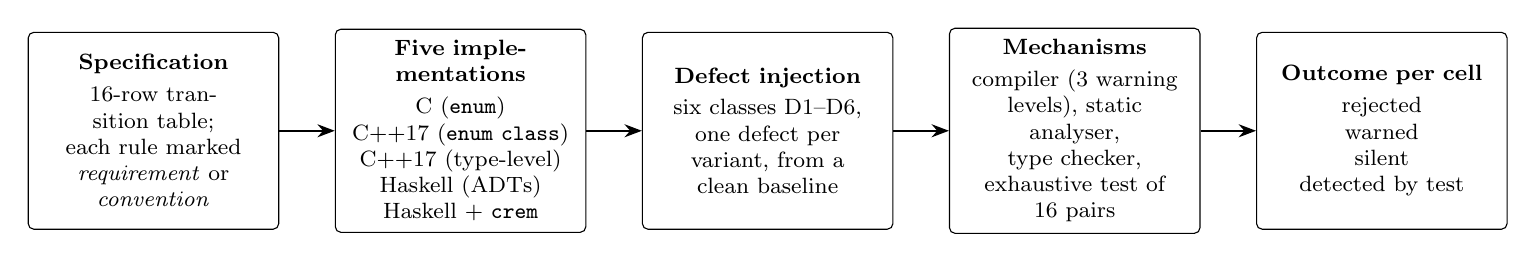
\begin{tikzpicture}[
    box/.style={draw, rounded corners=2pt, align=center, inner sep=4pt, text width=2.9cm, minimum height=2.5cm, font=\footnotesize},
    ar/.style={-{Stealth[length=2.2mm]}, thick}
]
\node[box] (spec) at (0,0) {\textbf{Specification}\\[2pt]16-row transition table;\\each rule marked\\\textit{requirement} or\\\textit{convention}};
\node[box] (impl) at (3.9,0) {\textbf{Five implementations}\\[2pt]C (\texttt{enum})\\C++17 (\texttt{enum class})\\C++17 (type-level)\\Haskell (ADTs)\\Haskell + \texttt{crem}};
\node[box] (def) at (7.8,0) {\textbf{Defect injection}\\[2pt]six classes D1--D6,\\one defect per\\variant, from a\\clean baseline};
\node[box] (mech) at (11.7,0) {\textbf{Mechanisms}\\[2pt]compiler (3 warning\\levels), static analyser,\\type checker,\\exhaustive test of\\16 pairs};
\node[box] (out) at (15.6,0) {\textbf{Outcome per cell}\\[2pt]rejected\\warned\\silent\\detected by test};
\draw[ar] (spec) -- (impl);
\draw[ar] (impl) -- (def);
\draw[ar] (def) -- (mech);
\draw[ar] (mech) -- (out);
\end{tikzpicture}
\end{document}
